\documentclass[landscape, 12pt]{beamer}

\usetheme{Madrid}
\usecolortheme{default}

\usepackage[utf8]{inputenc}
\usepackage[T1]{fontenc}
\usepackage[brazil]{babel}
\usepackage{graphicx}
\usepackage{amsmath,amssymb}
\usepackage{wasysym}
\usepackage{float}
\usepackage{xcolor}
\usepackage{hyperref}
\usepackage{tabularx}

\title{Análise de Crescimento de Plantas a Partir de Fotos Semanais}
\subtitle{Plant Growth Analyzer}
\author{
    Lucas Cardoso dos Santos \\
    Lucas Miranda Mendonça Rezende
}
\institute{Universidade de São Paulo - Ribeirão Preto}
\date{2025}

% Remove barra inferior e símbolos de navegação
\setbeamertemplate{footline}{}
\setbeamertemplate{navigation symbols}{}

\begin{document}

% Slide de título
\begin{frame}
    \titlepage
\end{frame}

% Slide de sumário
\begin{frame}{Sumário}
    \begin{enumerate}
        \item Introdução
        \item Requisitos
        \item Telas Principais
        \item Casos de Uso
        \item Inspeção de Usabilidade
        \item Teste de Usabilidade
        \item Testes Automáticos
        \item Conclusão
    \end{enumerate}
\end{frame}

% Seção: Introdução
\begin{frame}{Introdução}
    \begin{center}
        \textbf{Introdução}
    \end{center}
\end{frame}

\begin{frame}{O que é o Plant Growth Analyzer?}
    \begin{itemize}
        \item Aplicação desktop para análise de crescimento de plantas
        \item Desenvolvida em Angular e Electron
        \item Processa fotografias semanais automaticamente
        \item Extrai métricas: altura, largura e área
        \item Organiza dados em coleções
        \item Gera gráficos evolutivos de crescimento
    \end{itemize}
\end{frame}

\begin{frame}{Objetivo Principal}
    \textbf{Democratizar o acesso a técnicas de análise de crescimento vegetal}
    
    \vspace{0.5cm}
    \begin{itemize}
        \item Monitoramento regular através de fotos padronizadas
        \item Análise quantitativa automática com algoritmos de segmentação
        \item Organização eficiente de dados em coleções
        \item Visualização de tendências de crescimento ao longo do tempo
        \item Redução do trabalho manual de análise
    \end{itemize}
\end{frame}

\begin{frame}{Funcionalidades Principais}
    \begin{itemize}
        \item Upload individual e múltiplo de imagens
        \item Processamento automático com algoritmos de segmentação
        \item Configurações personalizáveis de processamento
        \item Organização em coleções temáticas
        \item Gráficos evolutivos de crescimento
        \item Edição pós-processamento de resultados
        \item Associação automática de datas
        \item Visualização lado a lado (original/processada)
    \end{itemize}
\end{frame}

% Seção: Requisitos
\begin{frame}{Requisitos}
    \begin{center}
        \textbf{Requisitos}
    \end{center}
\end{frame}

\begin{frame}{Requisitos de Imagens}
    \begin{itemize}
        \item Upload de uma ou mais imagens por vez
        \item Associação de imagens a coleções
        \item Configurações personalizáveis (granularidade, threshold)
        \item Associação de datas (metadados ou data atual)
        \item Visualização de resultados (imagem inicial, final e métricas)
        \item Edição pós-processamento de configurações e datas
        \item Exclusão de imagens
    \end{itemize}
\end{frame}

\begin{frame}{Requisitos de Coleções}
    \begin{itemize}
        \item Criação de novas coleções com nome
        \item Visualização de coleção e seus dados
        \item Acesso individual a cada imagem
        \item Acesso a gráficos de evolução temporal
        \item Exclusão de coleções existentes
        \item Renomeação de coleções
        \item Associação de imagens a coleções
        \item Remoção de imagens específicas de coleções
    \end{itemize}
\end{frame}

% Seção: Telas Principais
\begin{frame}{Telas Principais}
    \begin{center}
        \textbf{Telas Principais}
    \end{center}
\end{frame}

\begin{frame}{Telas Principais - Tela Principal}
    \begin{center}
        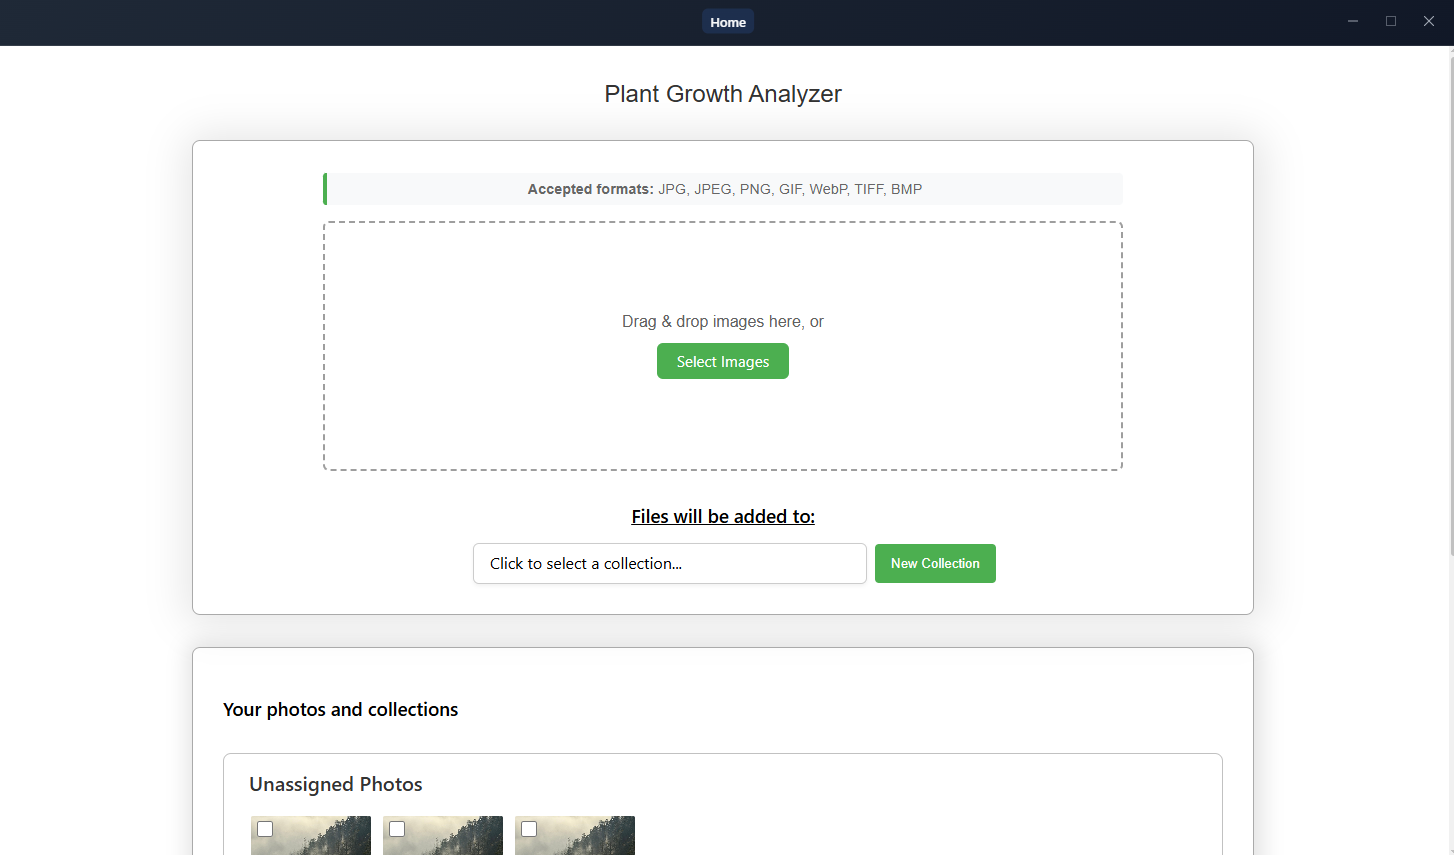
\includegraphics[width=0.9\textwidth]{../figures/hci/home_page.png}
    \end{center}
\end{frame}

\begin{frame}{Telas Principais - Visualizar Coleção}
    \begin{center}
        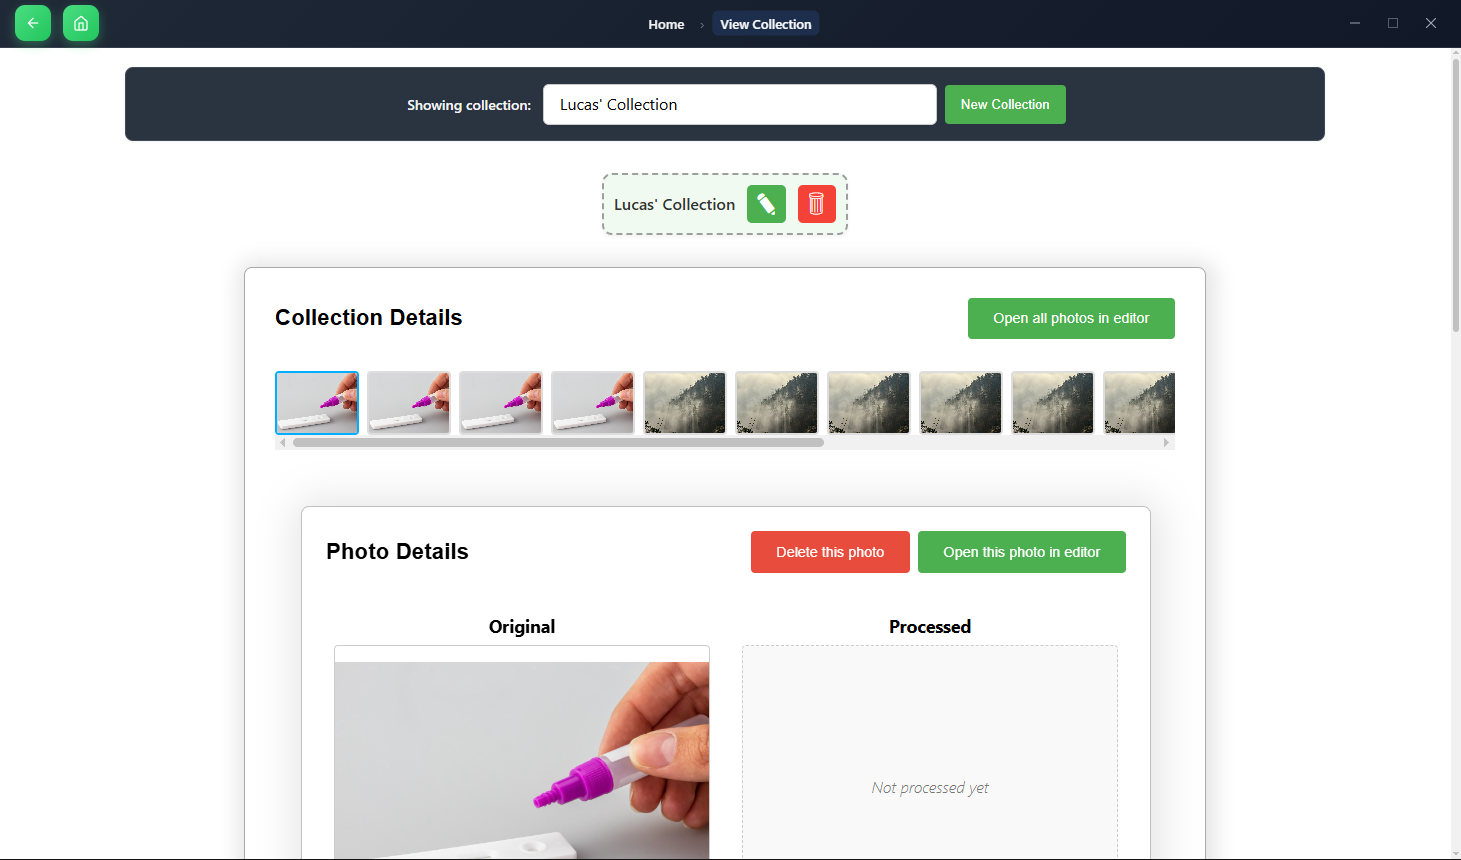
\includegraphics[width=0.9\textwidth]{../figures/hci/view_collection.png}
    \end{center}
\end{frame}

\begin{frame}{Telas Principais - Visualizar Foto}
    \begin{center}
        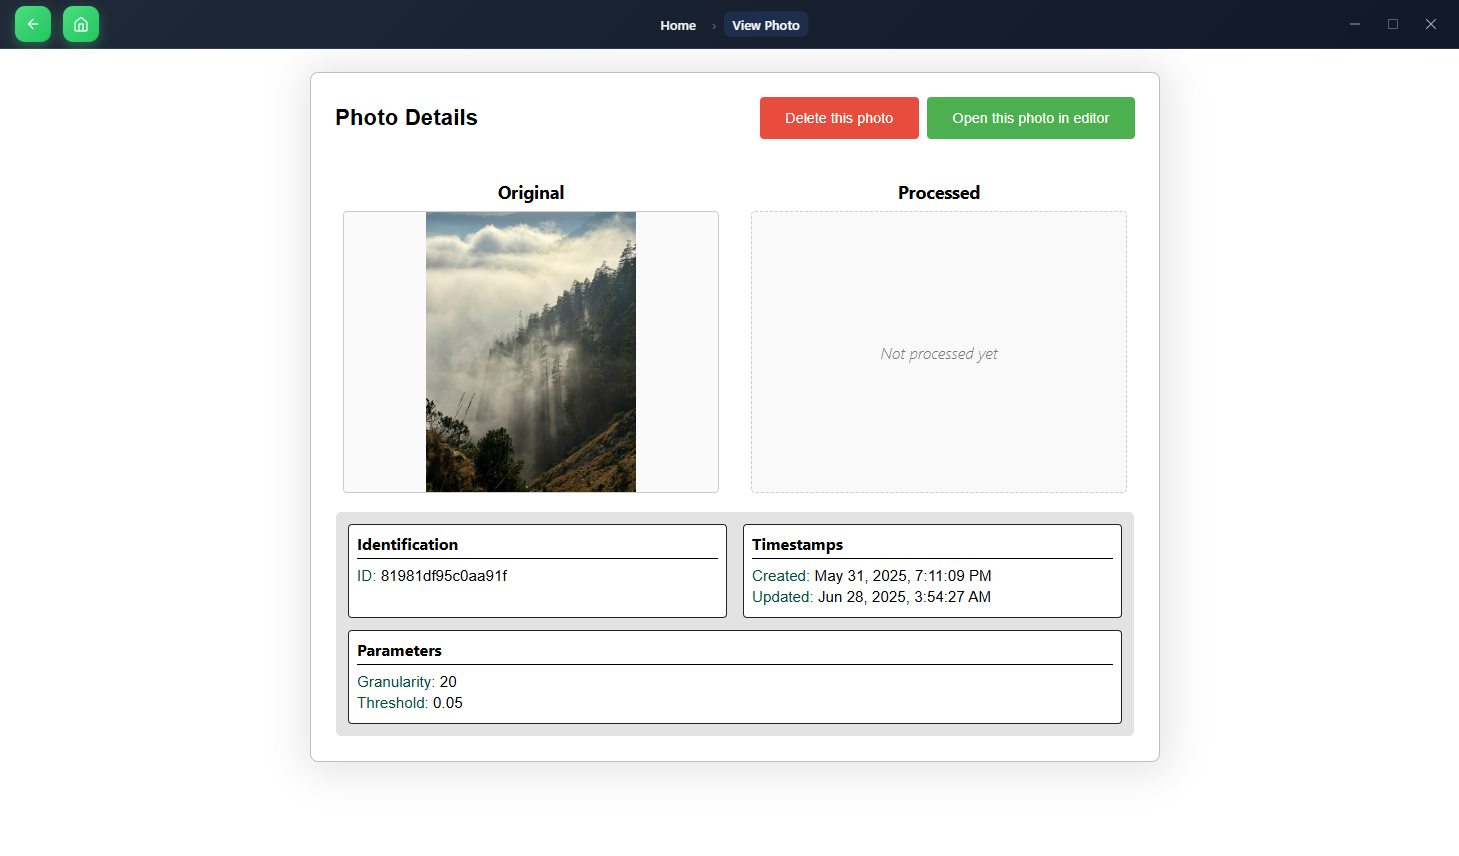
\includegraphics[width=0.9\textwidth]{../figures/hci/view_photo.png}
    \end{center}
\end{frame}

\begin{frame}{Telas Principais - Editar Foto}
    \begin{center}
        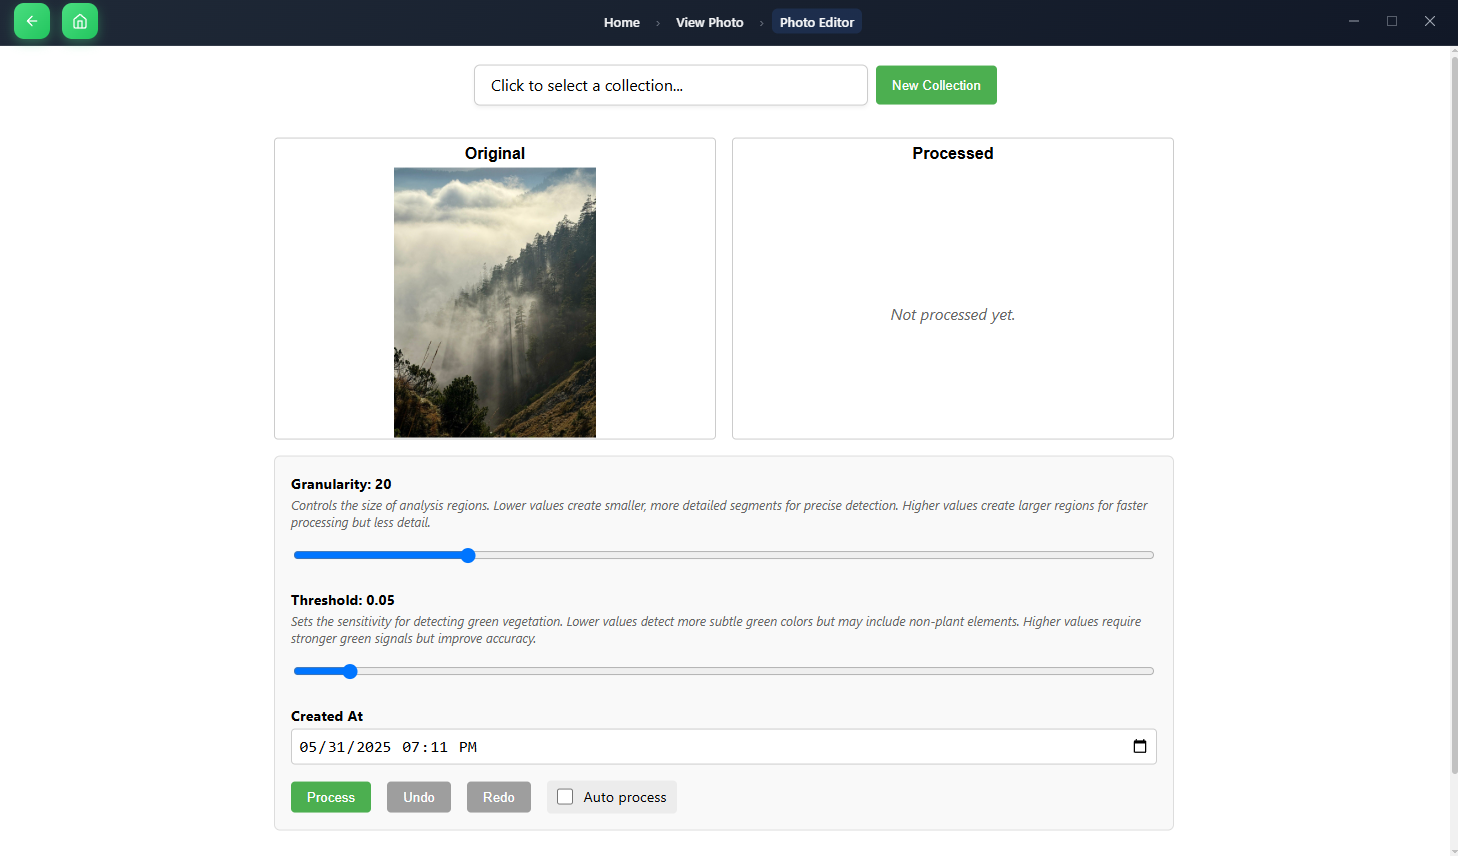
\includegraphics[width=0.9\textwidth]{../figures/hci/photo_editor.png}
    \end{center}
\end{frame}

% Seção: Casos de Uso
\begin{frame}{Casos de Uso}
    \begin{center}
        \textbf{Casos de Uso}
    \end{center}
\end{frame}

\begin{frame}{Casos de Uso Principais}
    \begin{itemize}
        \item Fazer envio de uma única foto
        \item Fazer envio de múltiplas imagens
        \item Adicionar foto à coleção
        \item Remover foto de coleção
        \item Deletar foto
        \item Visualizar detalhes de foto
        \item Processar foto única
        \item \textbf{Processar múltiplas fotos}
        \item Criar nova coleção
        \item Renomear coleção
        \item Deletar coleção
        \item Visualizar fotos de coleção
        \item Visualizar gráficos de crescimento
        \item Realizar operações de Desfazer/Refazer durante processamento
    \end{itemize}
\end{frame}

\begin{frame}{Processar Múltiplas Fotos - HTA Model}
    \begin{center}
        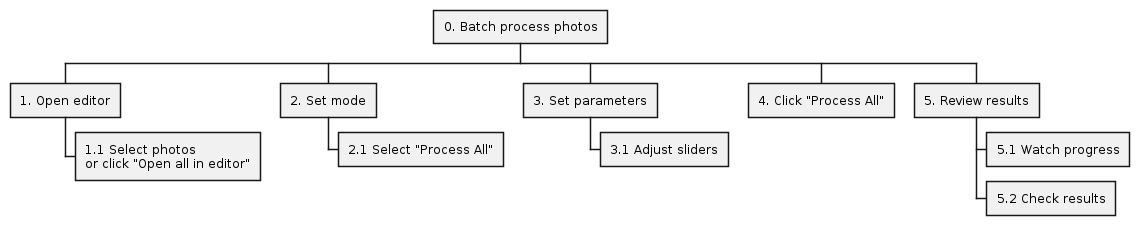
\includegraphics[width=0.85\textwidth]{../figures/hta/UC012.png}
    \end{center}
\end{frame}

\begin{frame}{Processar Múltiplas Fotos - Diagrama de Sequência}
    \begin{center}
        \resizebox{0.6\textwidth}{!}{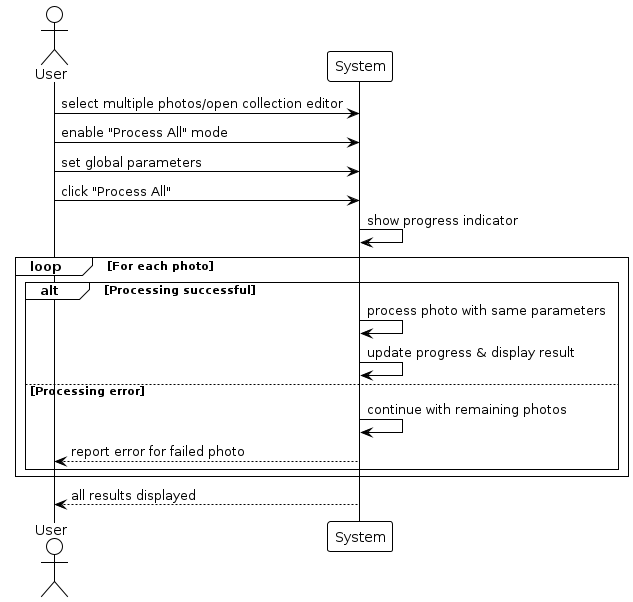
\includegraphics{../figures/dss/UC012.png}}
    \end{center}
\end{frame}

\begin{frame}{Processar Múltiplas Fotos}
    \begin{center}
        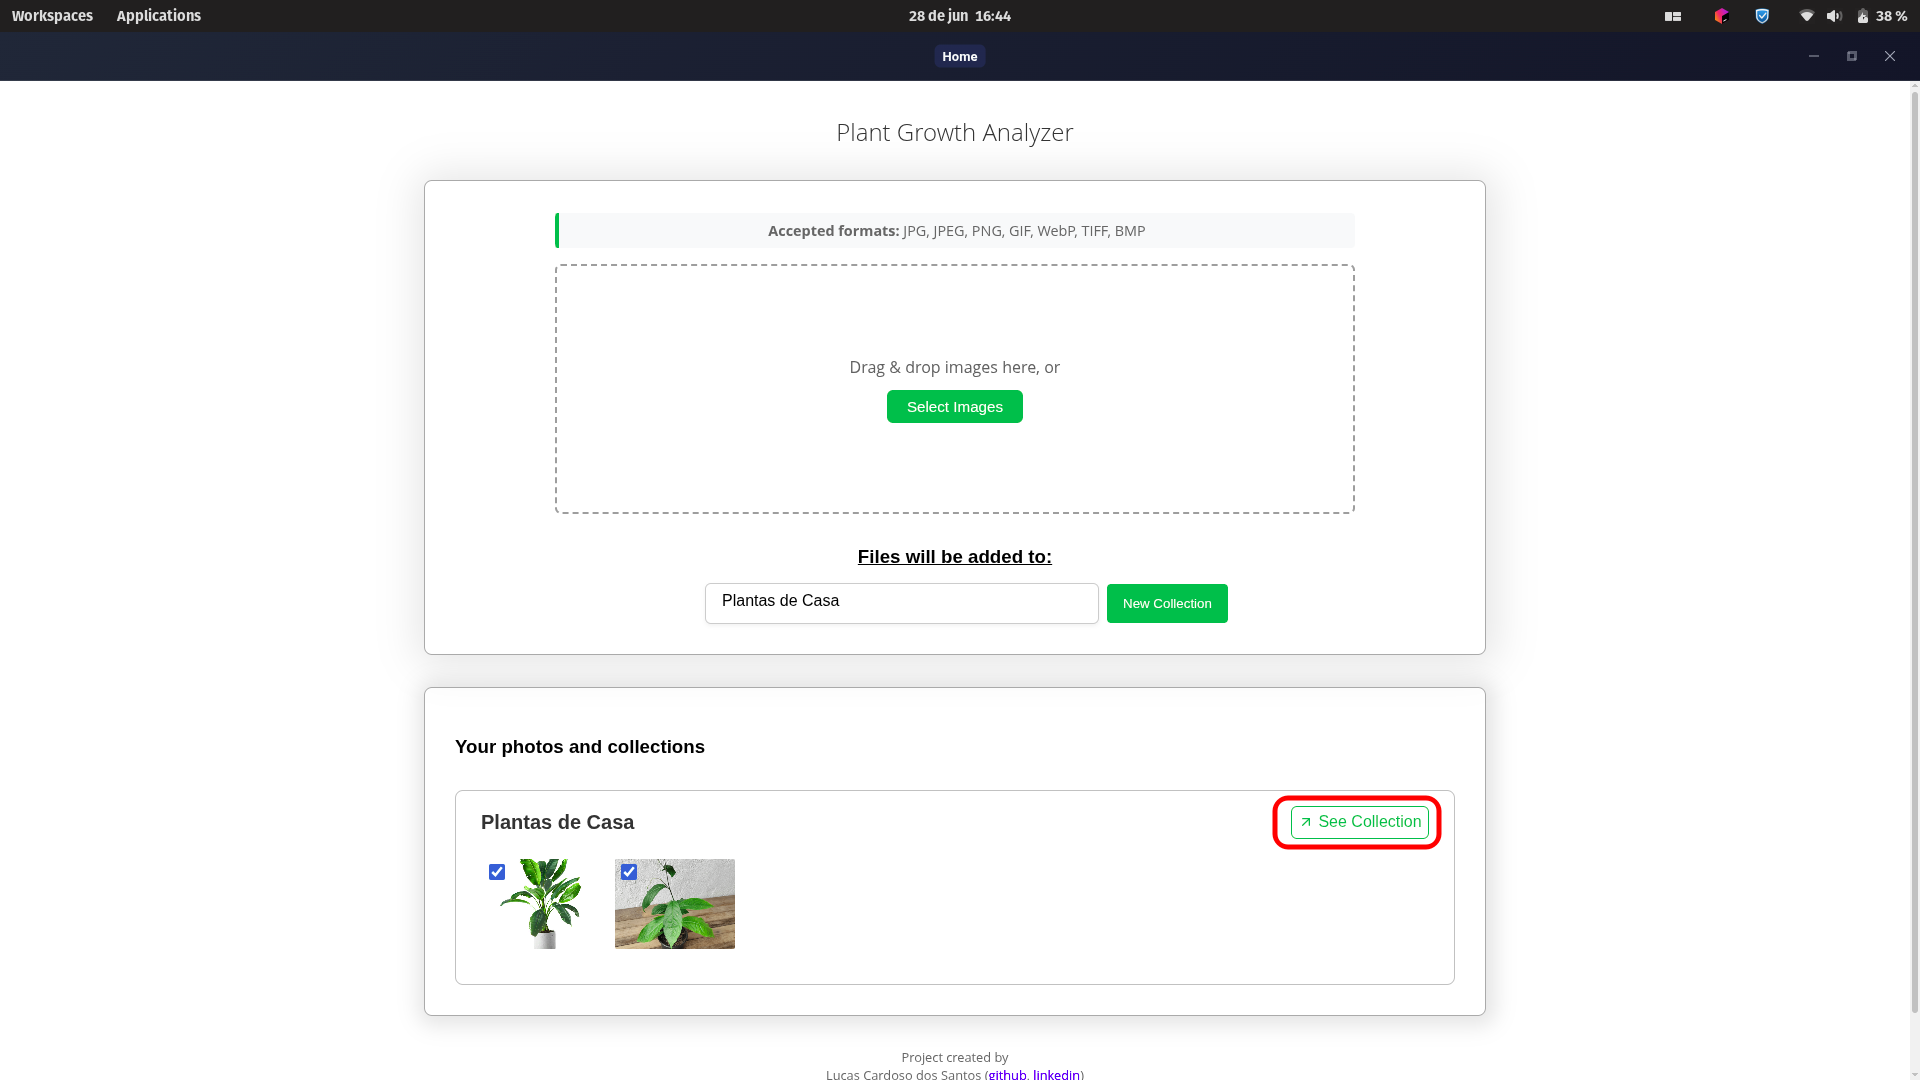
\includegraphics[width=0.95\textwidth]{../figures/screens/uc012/Screenshot from 2025-06-28 16-44-12.png}
    \end{center}
\end{frame}

\begin{frame}{Processar Múltiplas Fotos}
    \begin{center}
        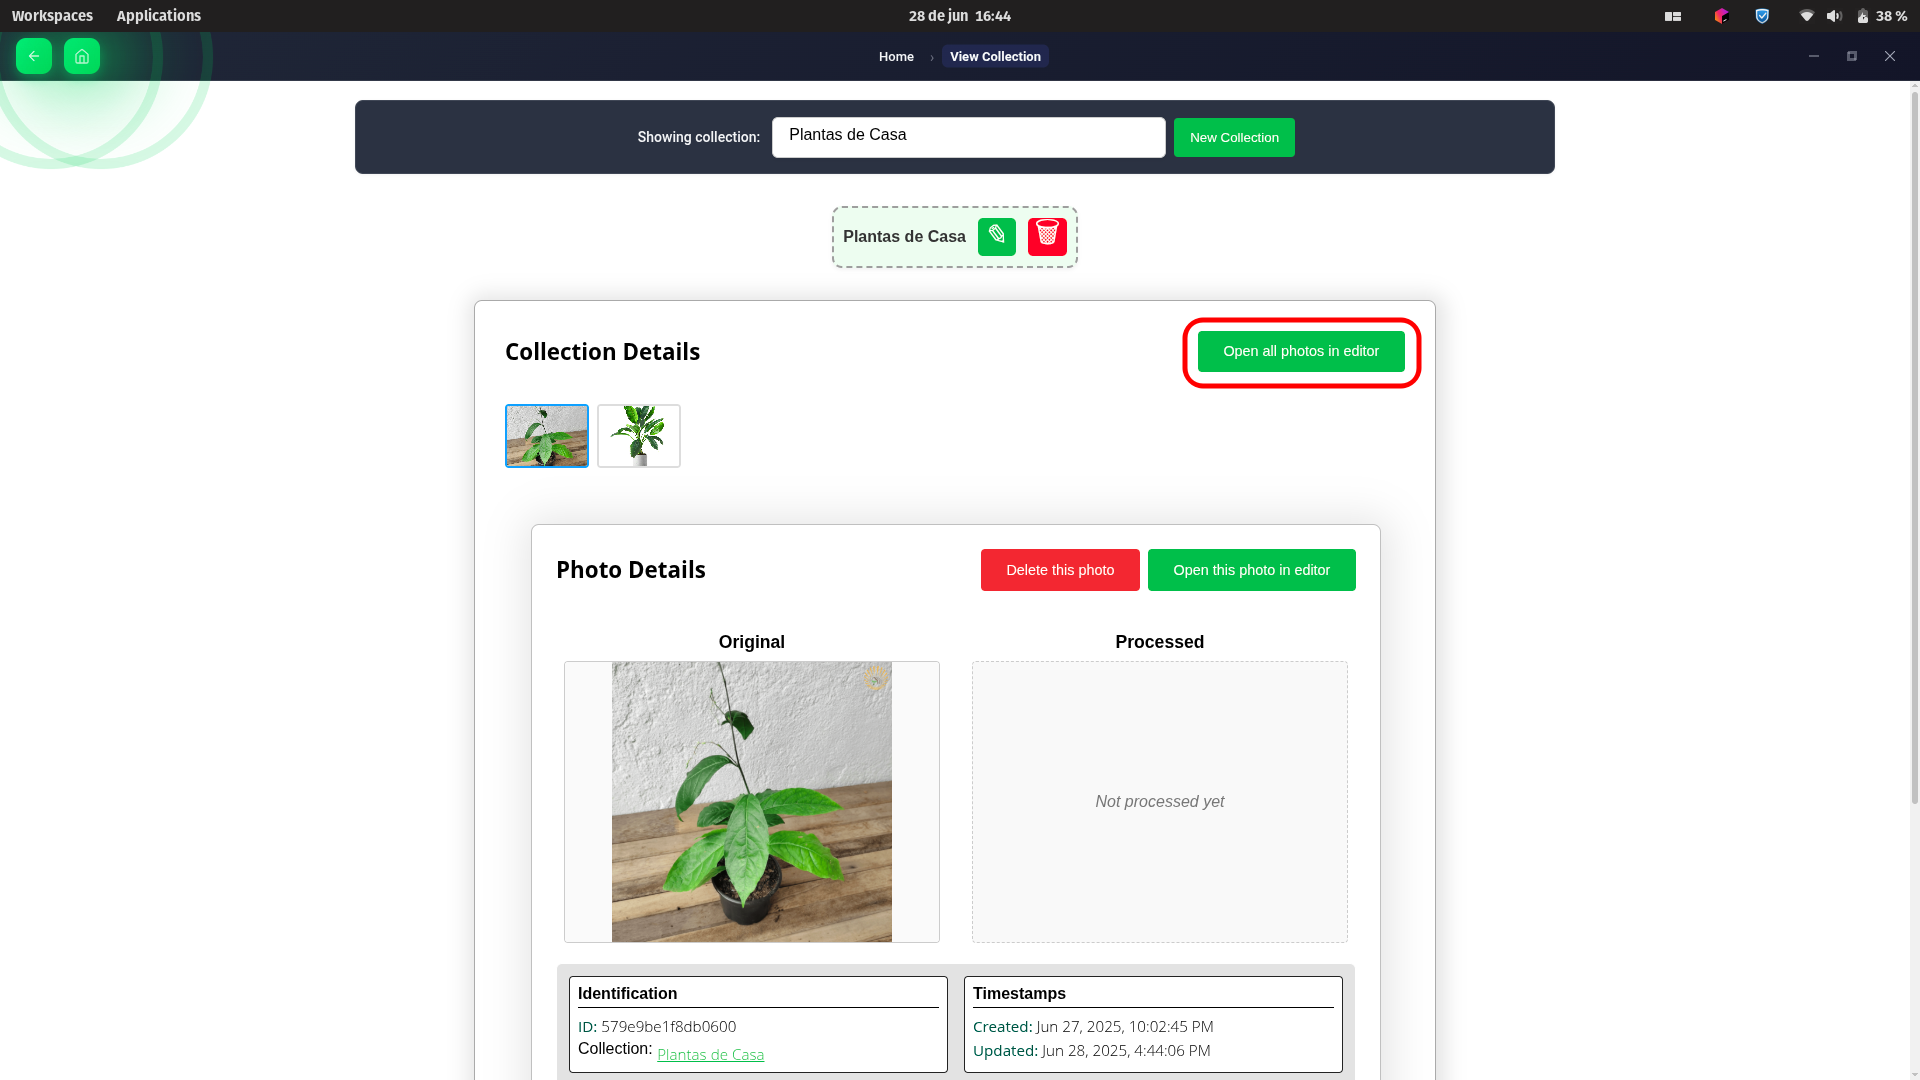
\includegraphics[width=0.95\textwidth]{../figures/screens/uc012/Screenshot from 2025-06-28 16-44-15.png}
    \end{center}
\end{frame}

\begin{frame}{Processar Múltiplas Fotos}
    \begin{center}
        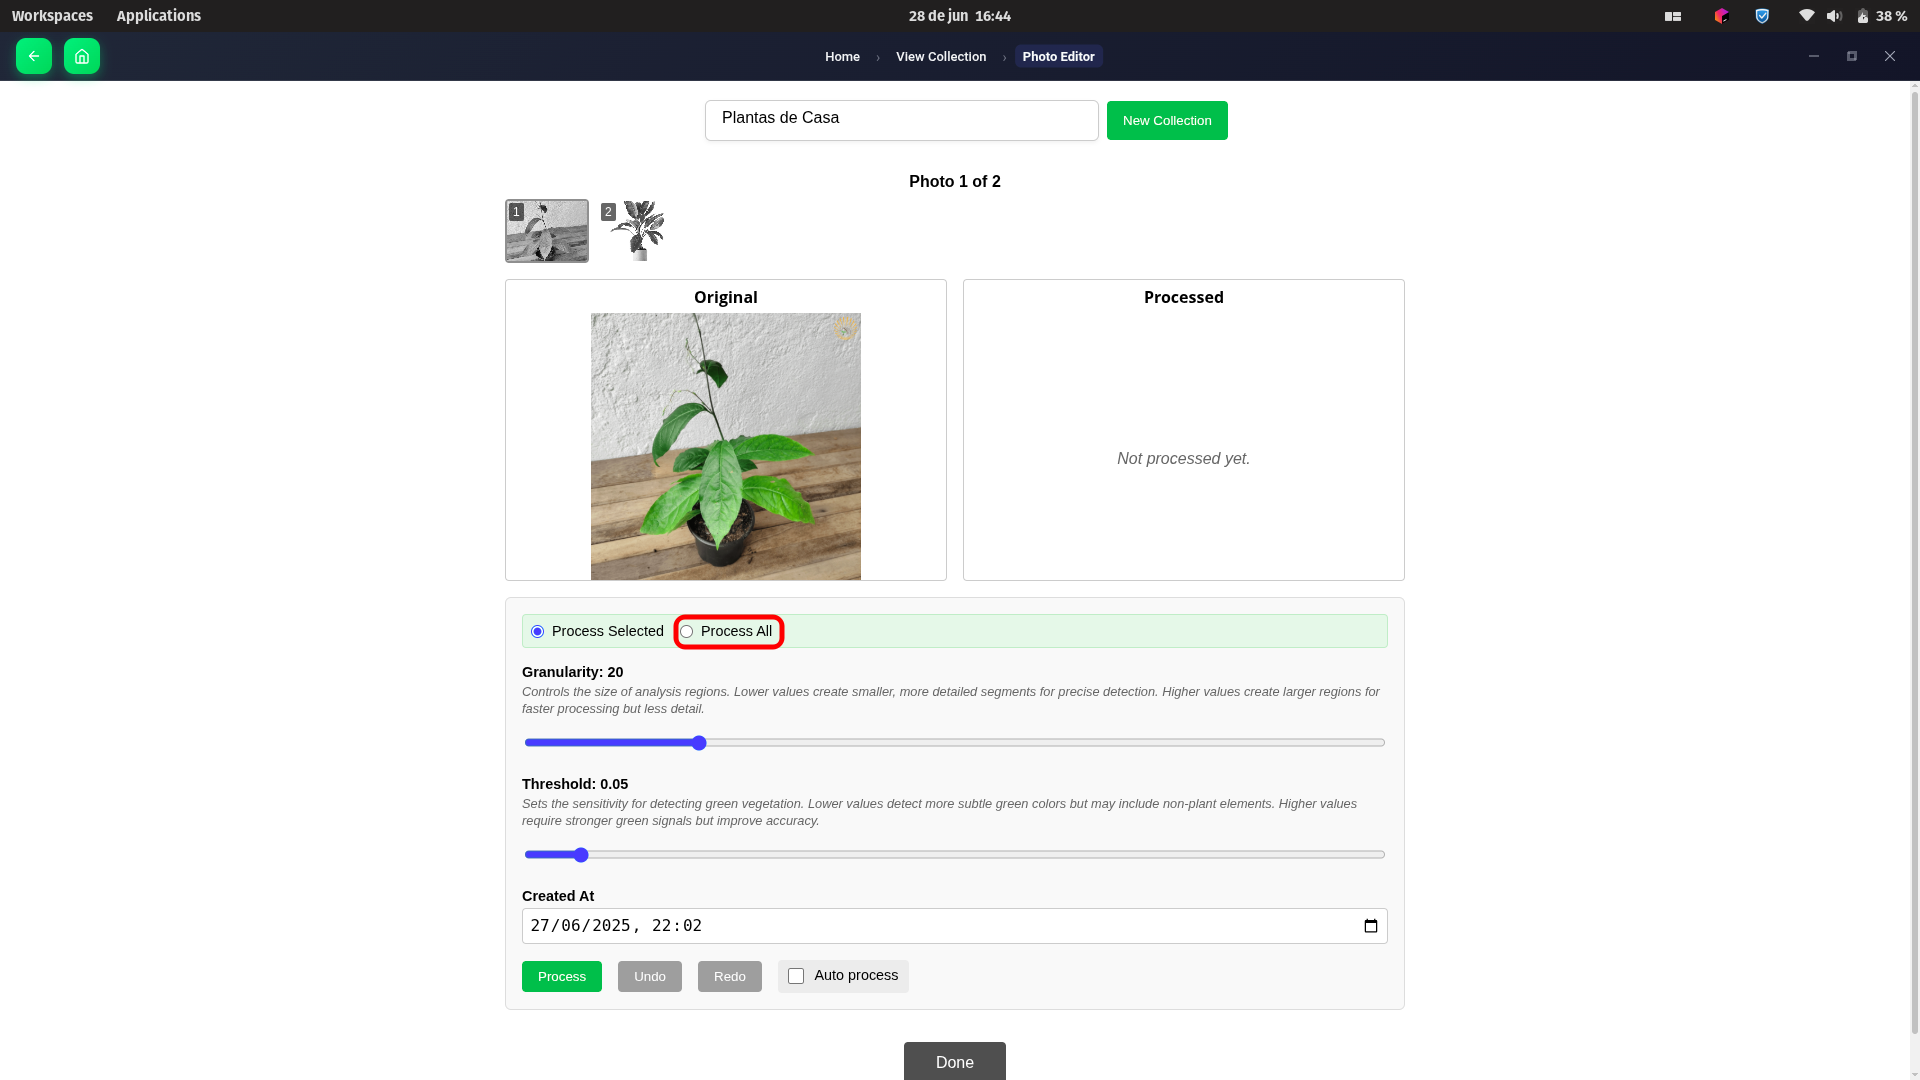
\includegraphics[width=0.95\textwidth]{../figures/screens/uc012/Screenshot from 2025-06-28 16-44-28.png}
    \end{center}
\end{frame}

\begin{frame}{Processar Múltiplas Fotos}
    \begin{center}
        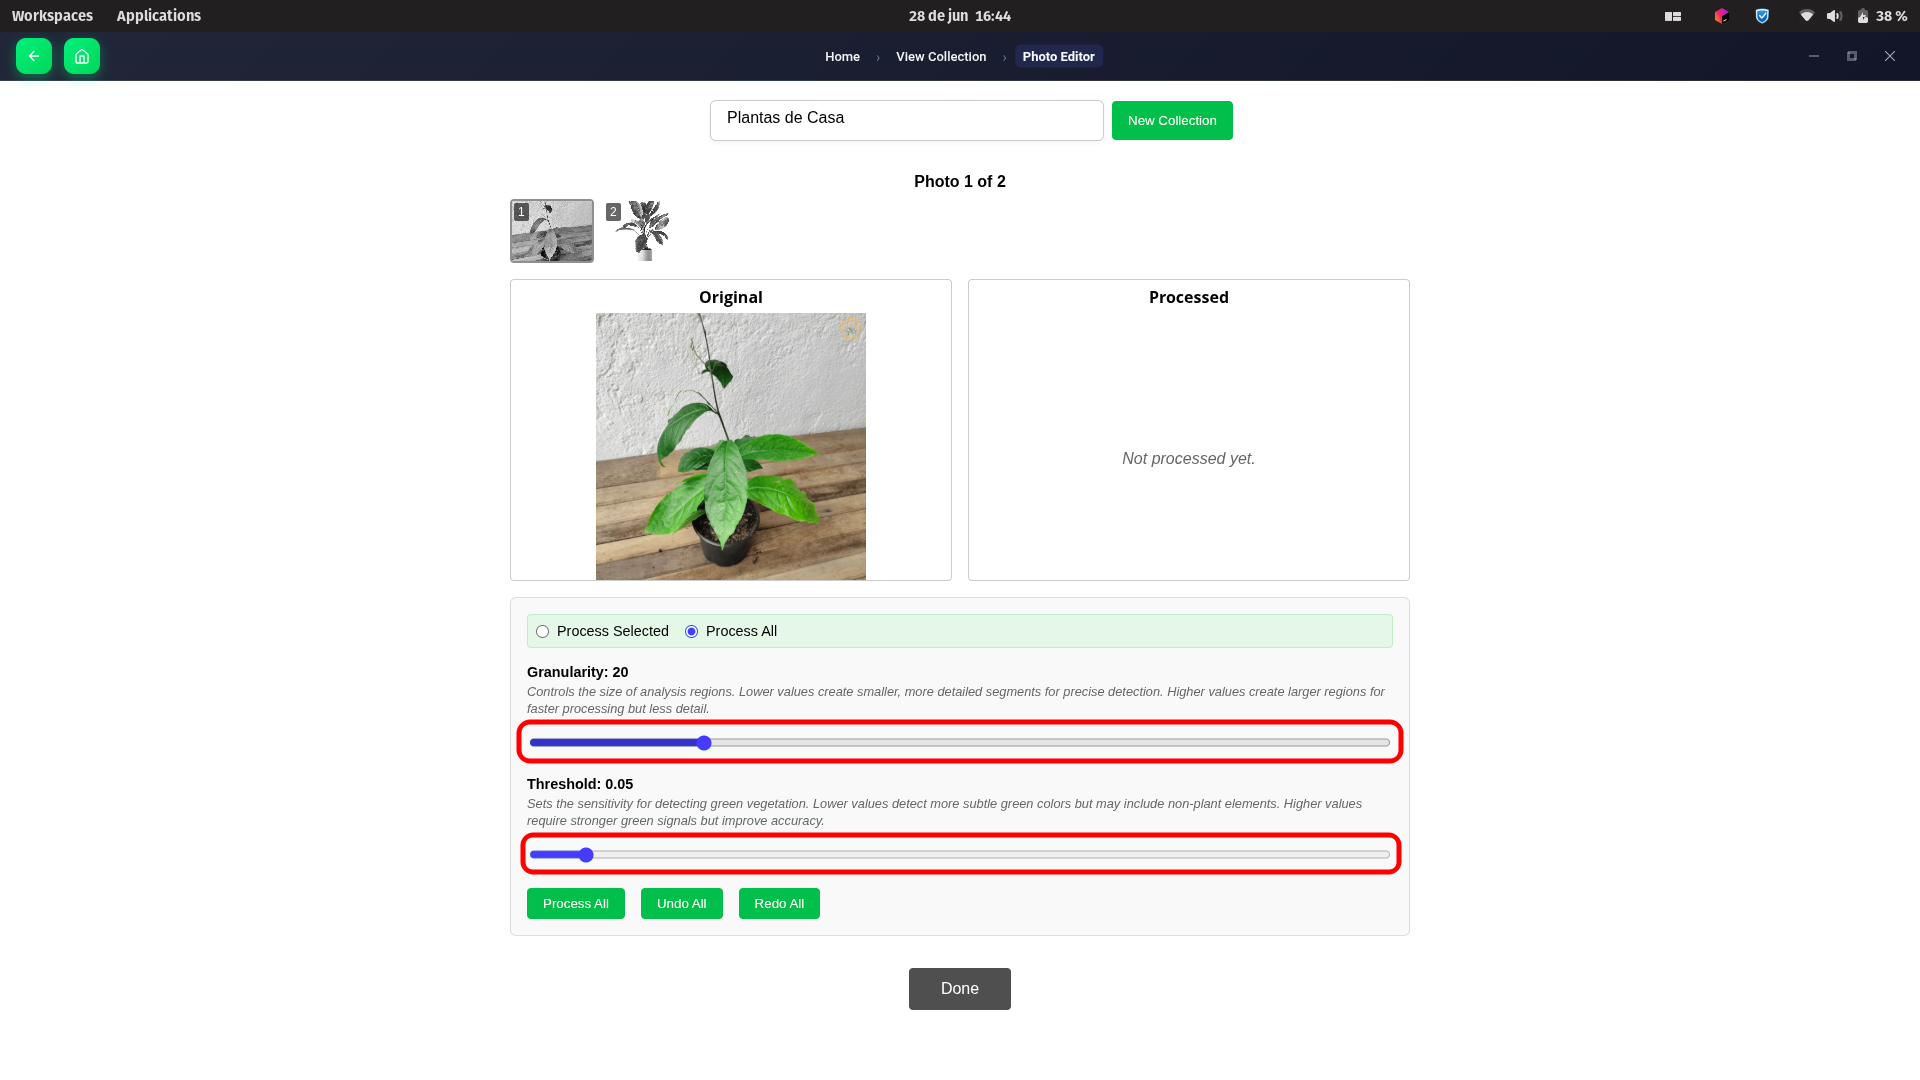
\includegraphics[width=0.95\textwidth]{../figures/screens/uc012/Screenshot from 2025-06-28 16-44-32.png}
    \end{center}
\end{frame}

\begin{frame}{Processar Múltiplas Fotos}
    \begin{center}
        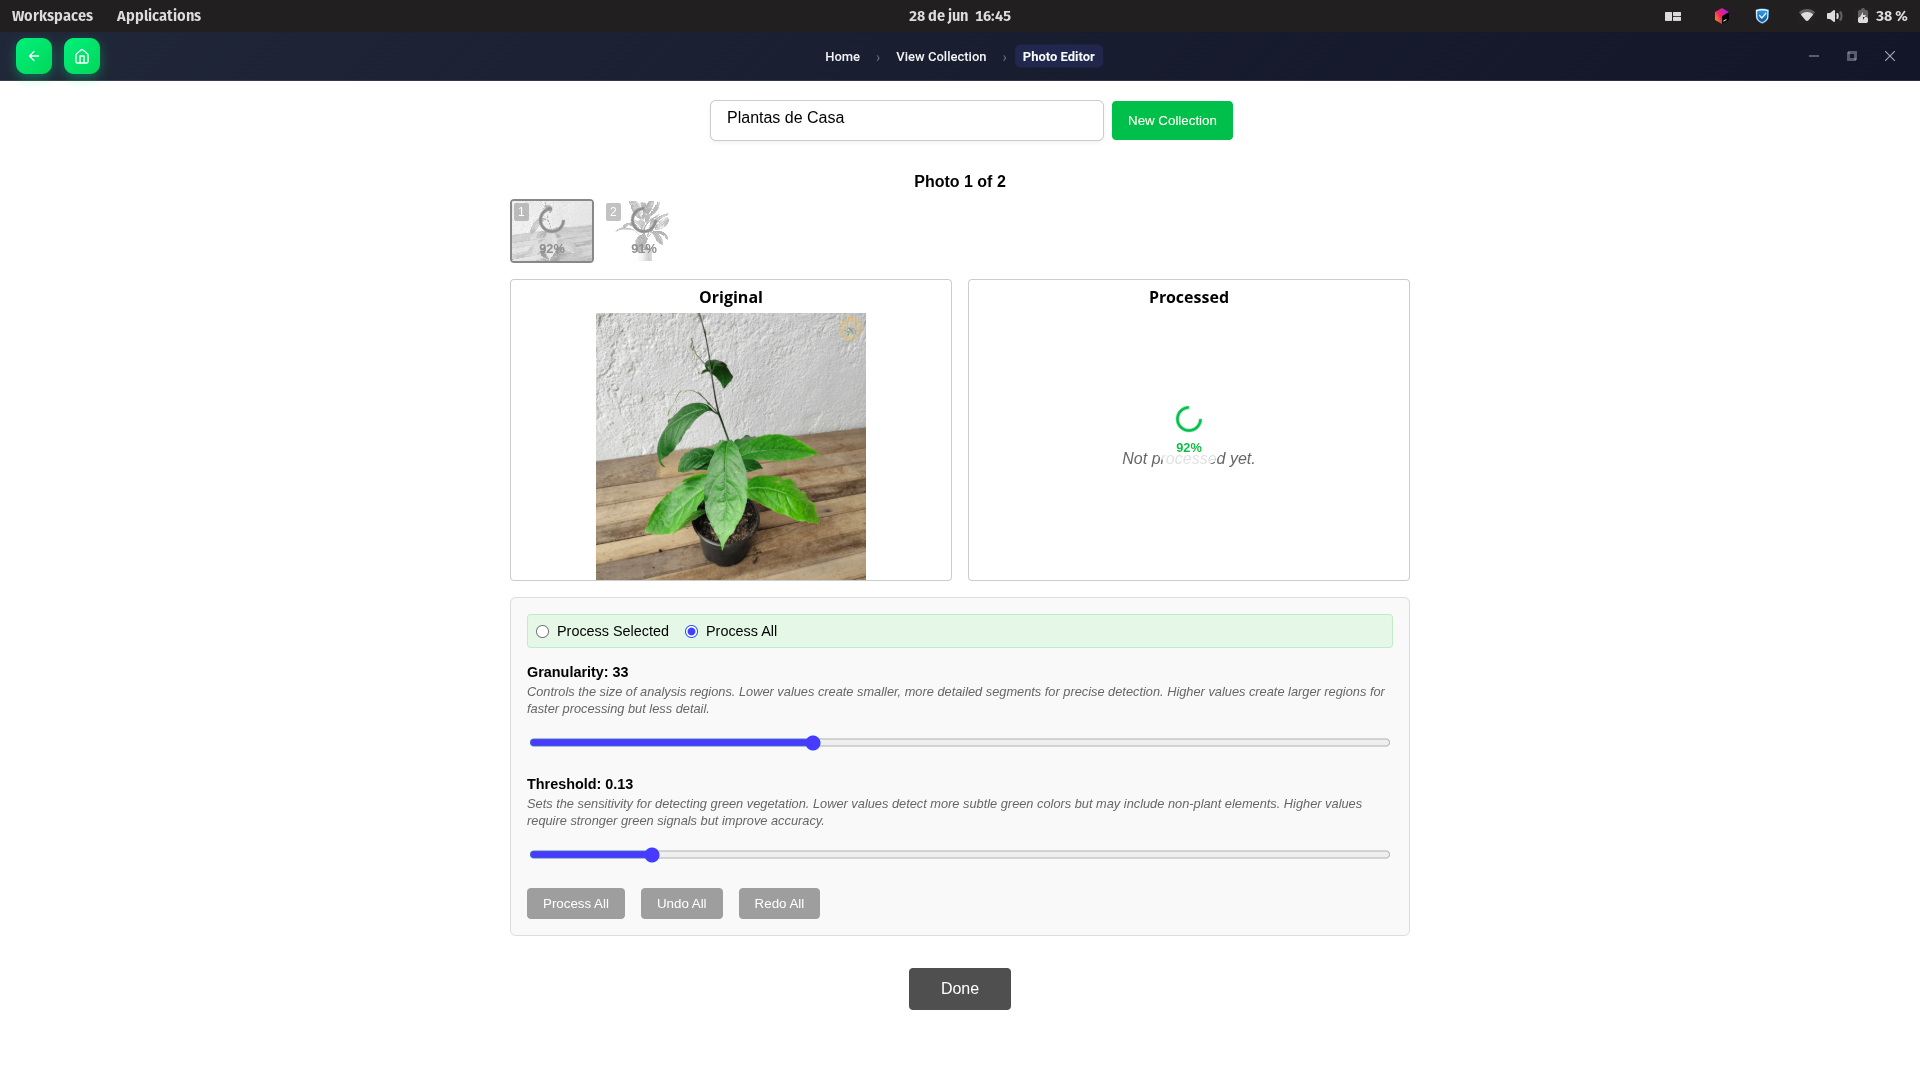
\includegraphics[width=0.95\textwidth]{../figures/screens/uc012/Screenshot from 2025-06-28 16-45-48.png} 
    \end{center}
\end{frame}

\begin{frame}{Processar Múltiplas Fotos}
    \begin{center}
        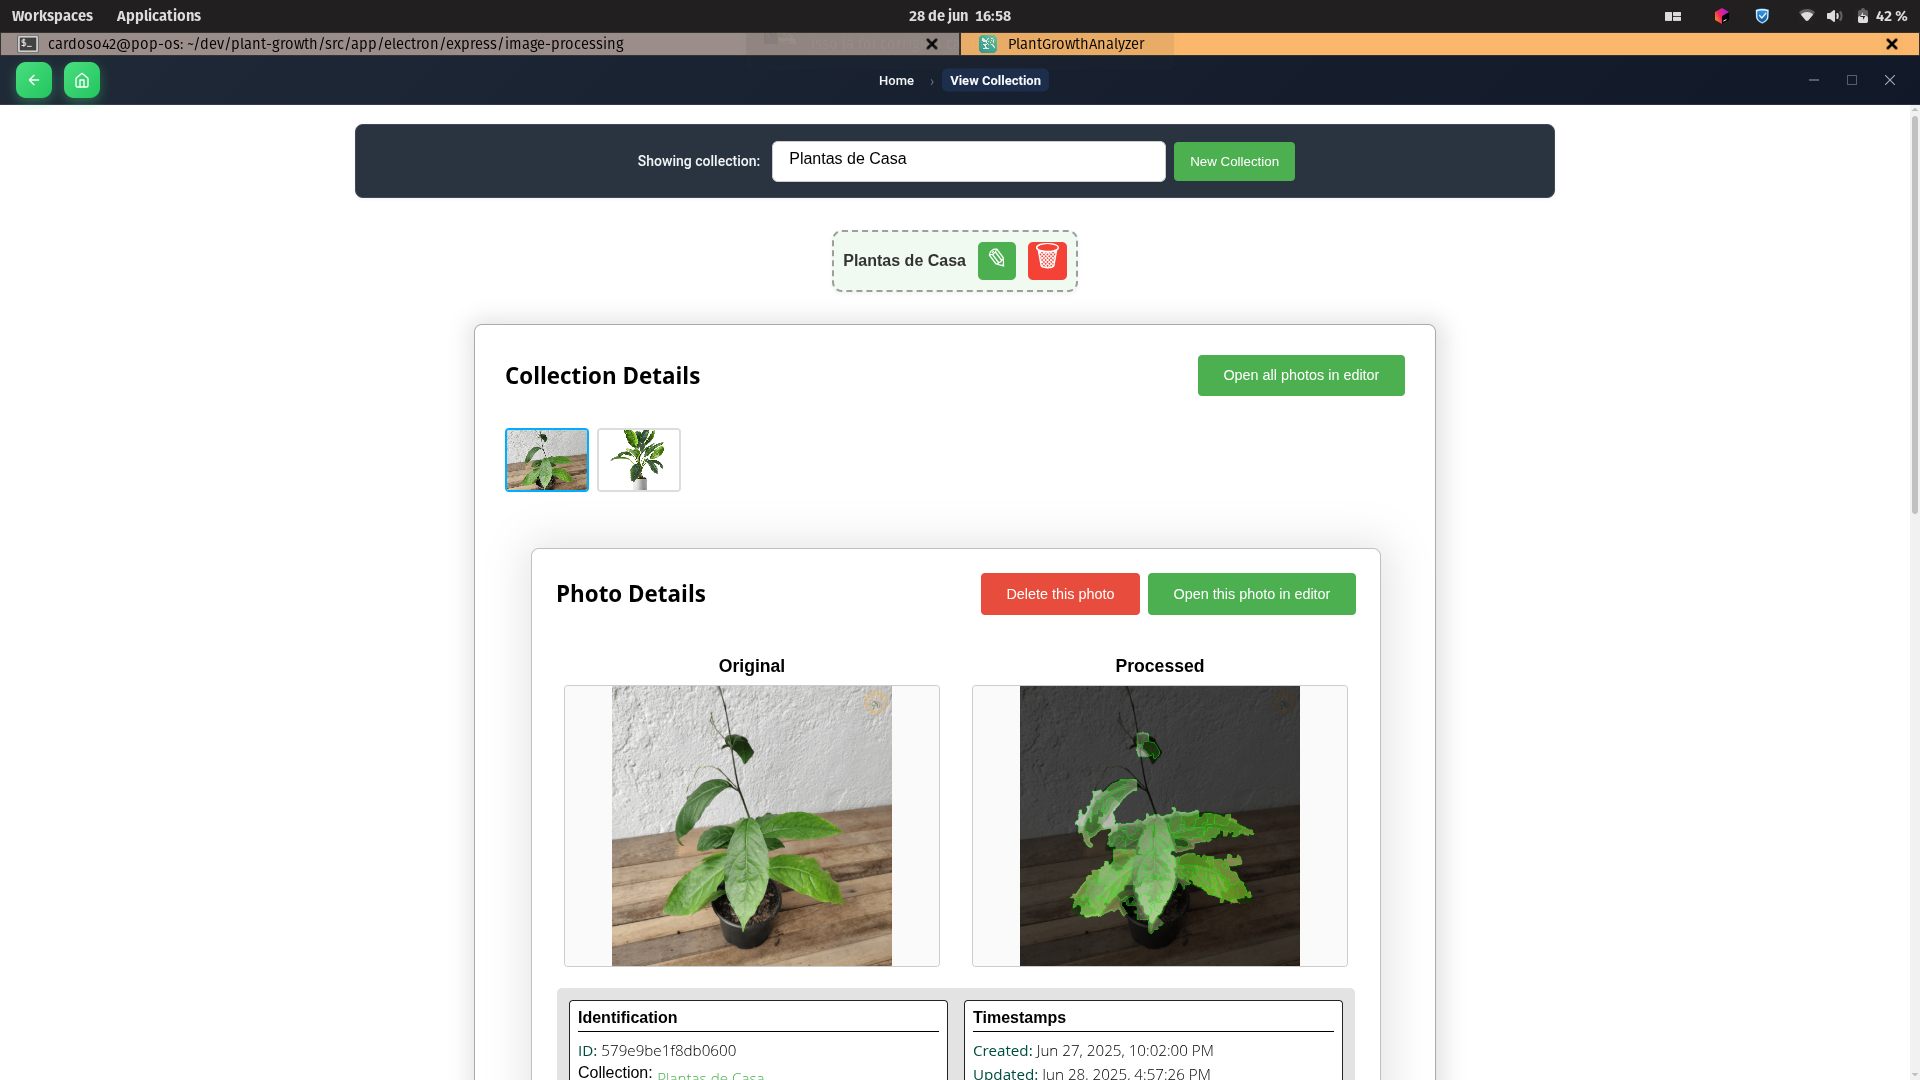
\includegraphics[width=0.95\textwidth]{../figures/screens/uc012/Screenshot from 2025-06-28 16-58-13.png}
    \end{center}
\end{frame}

% Seção: Inspeção de Usabilidade
\begin{frame}{Inspeção de Usabilidade}
    \begin{center}
        \textbf{Inspeção de Usabilidade}
    \end{center}
\end{frame}

\begin{frame}{Inspeção de Usabilidade - Metodologia}
    \begin{itemize}
        \item \textbf{5 avaliadores especialistas} em IHC
        \item \textbf{Avaliação Heurística de Nielsen} + \textbf{Princípios de Norman}
        \item Tempo: ~1h por avaliador
        \item Lista de tarefas específicas fornecida
        \item Formulário estruturado para avaliação
        \item \textbf{82 problemas identificados} no total
    \end{itemize}
\end{frame}

\begin{frame}{Inspeção de Usabilidade - Passo a Passo}
    \begin{itemize}
        \item 1. Escolha dos avaliadores (perfil e experiência)
        \item 2. Familiarização com o sistema
        \item 3. Execução de tarefas pré-definidas
        \item 4. Preenchimento de formulário estruturado
        \item 5. Coleta de comentários e problemas
        \item 6. Discussão e agregação dos resultados
        \item 7. Classificação dos problemas por gravidade
    \end{itemize}
\end{frame}

\begin{frame}{Inspeção de Usabilidade - Escolha dos Avaliadores}
    \begin{itemize}
        \item Avaliadores: docentes e discentes de Ciência da Computação
        \item Experiência prévia em avaliação heurística
        \item Diversidade de perfis para maior abrangência
    \end{itemize}
\end{frame}

\begin{frame}{Inspeção de Usabilidade - Execução das Tarefas}
    \begin{itemize}
        \item Cada avaliador recebeu lista de tarefas representativas
        \item Utilização livre do sistema para explorar funcionalidades
        \item Preenchimento de formulário com base nas heurísticas e princípios
    \end{itemize}
\end{frame}

\begin{frame}{Inspeção de Usabilidade - Coleta e Discussão}
    \begin{itemize}
        \item Coleta de comentários únicos e relevantes
        \item Discussão coletiva para agregar avaliações
        \item Classificação dos problemas encontrados
    \end{itemize}
\end{frame}

\begin{frame}{Inspeção de Usabilidade - Problemas por Gravidade}
    \begin{center}
        \begin{tabularx}{0.95\textwidth}{|c|c|X|}
            \hline
            \textbf{Gravidade} & \textbf{Qtd} & \textbf{Descrição} \\
            \hline
            4 (Catastrófico) & 2 & Falta de confirmação para exclusão \\
            \hline
            3 (Grave) & 5 & Inconsistência visual, navegação confusa \\
            \hline
            2 (Moderado) & 4 & Controle limitado, jargão técnico \\
            \hline
            1 (Menor) & 2 & Funcionalidades de gráficos \\
            \hline
        \end{tabularx}
    \end{center}
\end{frame}

\begin{frame}{Inspeção de Usabilidade - Problemas Críticos}
    \begin{itemize}
        \item \textbf{Consistência Visual} (22\%): Cores e posicionamento inconsistentes
        \item \textbf{Prevenção de Erros} (16\%): Falta de confirmações para ações destrutivas
        \item \textbf{Visibilidade do Status} (15\%): Feedback inadequado durante operações
        \item \textbf{Reconhecimento vs. Lembrança} (15\%): Interface não autoexplicativa
    \end{itemize}
\end{frame}

\begin{frame}{Inspeção de Usabilidade - Recomendações}
    \begin{itemize}
        \item \textbf{Alta Prioridade}:
        \begin{itemize}
            \item Implementar confirmações para exclusões
            \item Adicionar indicadores de progresso visíveis
            \item Corrigir mensagens de erro que desaparecem
        \end{itemize}
        \item \textbf{Média Prioridade}:
        \begin{itemize}
            \item Padronizar cores e posicionamento de botões
            \item Melhorar estrutura de navegação
            \item Adicionar rótulos descritivos para ícones
        \end{itemize}
    \end{itemize}
\end{frame}

% Seção: Teste de Usabilidade
\begin{frame}{Teste de Usabilidade}
    \begin{center}
        \textbf{Teste de Usabilidade}
    \end{center}
\end{frame}

\begin{frame}{Teste de Usabilidade - Metodologia}
    \begin{itemize}
        \item 5 participantes (estudantes e usuários web)
        \item Técnica Think Aloud durante execução
        \item 9 tarefas principais representativas
        \item Questionário Likert (1-5) de satisfação
        \item Duração: 30-60 minutos por sessão
        \item Acompanhamento por avaliador durante todo o processo
    \end{itemize}
\end{frame}

\begin{frame}{Teste de Usabilidade - Passo a Passo}
    \begin{itemize}
        \item 1. Escolha dos participantes (perfil e experiência)
        \item 2. Apresentação do sistema e instruções
        \item 3. Execução das tarefas pré-definidas
        \item 4. Aplicação da técnica Think Aloud
        \item 5. Preenchimento do questionário de satisfação
        \item 6. Coleta de comentários e dificuldades
        \item 7. Discussão e agregação dos resultados
    \end{itemize}
\end{frame}

\begin{frame}{Teste de Usabilidade - Escolha dos Participantes}
    \begin{itemize}
        \item Participantes: estudantes de graduação e usuários com experiência em aplicações web
        \item Diversidade de experiências técnicas
        \item Todos utilizam computadores regularmente
    \end{itemize}
\end{frame}

\begin{frame}{Teste de Usabilidade - Execução das Tarefas}
    \begin{itemize}
        \item Cada participante recebeu uma lista de tarefas representativas
        \item Execução livre das tarefas, sem interferência do avaliador
        \item Aplicação da técnica Think Aloud durante todo o processo
    \end{itemize}
\end{frame}

\begin{frame}{Teste de Usabilidade - Coleta e Discussão}
    \begin{itemize}
        \item Coleta de dados quantitativos (taxa de sucesso, tempo, erros)
        \item Coleta de dados qualitativos (comentários, dificuldades, sugestões)
        \item Discussão coletiva para agregar avaliações
        \item Análise dos resultados e recomendações
    \end{itemize}
\end{frame}

\begin{frame}{Teste de Usabilidade - Taxa de Sucesso por Tarefa}
    \begin{center}
        \begin{tabular}{|l|c|}
            \hline
            \textbf{Tarefa} & \textbf{Taxa de Sucesso} \\
            \hline
            Adicionar imagem & 100\% \\
            Processar imagem & 80\% \\
            Remover imagem & 100\% \\
            Editar imagem & 60\% \\
            Criar coleção & 100\% \\
            Associar imagem & 80\% \\
            Excluir coleção & 100\% \\
            \hline
        \end{tabular}
    \end{center}
\end{frame}

\begin{frame}{Teste de Usabilidade - Avaliação de Satisfação}
    \begin{center}
        \begin{tabular}{|l|c|}
            \hline
            \textbf{Aspecto} & \textbf{Média (1-5)} \\
            \hline
            Sistema fácil de usar & 3,8 \\
            Funcionalidades organizadas logicamente & 4,4 \\
            Confiança ao usar o sistema & 4,0 \\
            Linguagem clara e compreensível & 4,8 \\
            Aparência agradável & 4,4 \\
            Feedback suficiente sobre ações & 4,2 \\
            Dificuldade para concluir tarefas & 2,4 \\
            Compreensão dos resultados & 4,6 \\
            \hline
        \end{tabular}
    \end{center}
\end{frame}

\begin{frame}{Teste de Usabilidade - Principais Dificuldades}
    \begin{itemize}
        \item Clareza do fluxo de ações: necessidade de abrir no editor para processar
        \item Interação e affordance: botões apenas com ícones causam incerteza
        \item Feedback inadequado: ausência de mensagens claras de conclusão
        \item Consistência visual: padronização insuficiente de elementos
        \item Navegação confusa: posição de botões "voltar" pouco visível
    \end{itemize}
\end{frame}

\begin{frame}{Teste de Usabilidade - Recomendações}
    \begin{itemize}
        \item Feedback: exibir mensagens claras após operações
        \item Consistência: padronizar estilo e posição de botões
        \item Navegação: tornar mais evidente o caminho de ações principais
        \item Interface: incluir suporte a ações em lote
        \item Documentação: adicionar textos explicativos nos botões
    \end{itemize}
\end{frame}

% Seção: Testes Automáticos
\begin{frame}{Testes Automáticos}
    \begin{center}
        \textbf{Testes Automáticos}
    \end{center}
    \vspace{0.5cm}
    \begin{itemize}
        \item Avaliação sistemática da aplicação usando o Lighthouse
        \item Três modos: Navegação, Snapshot e Timespan
    \end{itemize}
    \vspace{0.5cm}
    \begin{center}
        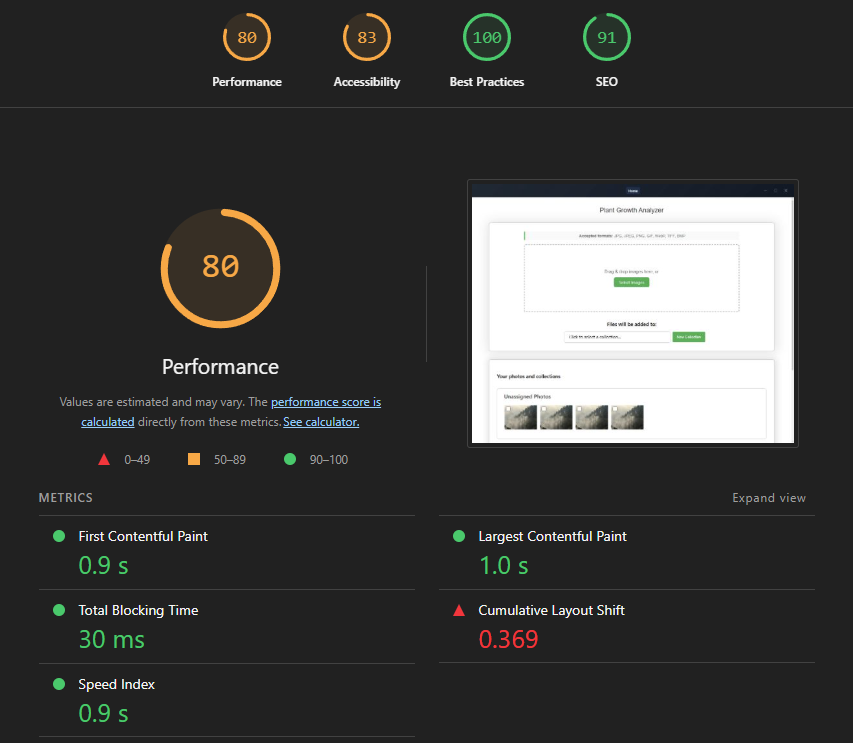
\includegraphics[width=0.7\textwidth]{../figures/hci/testes_automaticos.png}
    \end{center}
\end{frame}

\begin{frame}{Testes Automáticos - Metodologia}
    \begin{itemize}
        \item Ambiente controlado: Windows 10, Chrome 138, Lighthouse 12.6.0
        \item Testes realizados em http://localhost:3999/
        \item Modos:
        \begin{itemize}
            \item \textbf{Navegação}: simula carregamento completo da página
            \item \textbf{Snapshot}: captura instantânea do estado da interface
            \item \textbf{Timespan}: monitora desempenho durante uso contínuo
        \end{itemize}
    \end{itemize}
\end{frame}

\begin{frame}{Testes Automáticos - Navegação}
    \textbf{Foco:}
    \begin{itemize}
        \item Desempenho de carregamento, estabilidade visual, boas práticas
    \end{itemize}
    \vspace{0.3cm}
    \textbf{Principais Métricas:}
    \begin{table}[h]
    \centering
    \scriptsize
    \begin{tabular}{|l|c|c|c|c|}
    \hline
    \textbf{Métrica} & \textbf{Valor} & \textbf{Pontuação} & \textbf{Classificação} & \textbf{Benchmark} \\
    \hline
    FCP & 850.86 ms & 0.93 & Excelente & < 934 ms \\
    LCP & 1015.80 ms & 0.94 & Excelente & < 1200 ms \\
    Speed Index & 850.86 ms & 0.99 & Excelente & < 1311 ms \\
    CLS & 0.369 & 0.96 & Excelente & < 0.1 \\
    FID & 34.47 ms & 0.96 & Excelente & < 100 ms \\
    TTI & 1026.28 ms & 0.96 & Excelente & < 3500 ms \\
    TBT & 72 ms & 0.96 & Excelente & < 200 ms \\
    \hline
    \end{tabular}
    \end{table}
\end{frame}

\begin{frame}{Testes Automáticos - Navegação (Acessibilidade)}
    \textbf{Acessibilidade:}
    \begin{table}[h]
    \centering
    \scriptsize
    \begin{tabular}{|l|c|c|c|}
    \hline
    \textbf{Categoria} & \textbf{Status} & \textbf{Detalhes} & \textbf{Impacto} \\
    \hline
    Contraste de Cores & \textcolor{red}{Problema} & Contraste de 2.77 em botões & Baixo \\
    Estrutura Semântica & \textcolor{green}{Adequado} & Uso correto de elementos HTML & Alto \\
    Atributos ARIA & \textcolor{green}{Adequado} & Implementação correta & Alto \\
    Navegação por Teclado & \textcolor{green}{Adequado} & Funcionalidade completa & Alto \\
    \hline
    \end{tabular}
    \end{table}
\end{frame}

\begin{frame}{Testes Automáticos - Navegação (Boas Práticas)}
    \textbf{Boas Práticas e Segurança:}
    \begin{itemize}
        \item HTTPS: Não se aplica (Score: 1.0)
        \item Console Errors: Nenhum erro detectado (Score: 1.0)
        \item APIs Obsoletas: Não utilizadas (Score: 1.0)
        \item Viewport Meta Tag: Configurado adequadamente (Score: 1.0)
    \end{itemize}
\end{frame}

\begin{frame}{Testes Automáticos - Snapshot}
    \textbf{Foco:}
    \begin{itemize}
        \item Acessibilidade, contraste, estado da interface
    \end{itemize}
    \vspace{0.3cm}
    \textbf{Resultados:}
    \begin{table}[h]
    \centering
    \scriptsize
    \begin{tabular}{|l|c|c|c|}
    \hline
    \textbf{Elemento} & \textbf{Status} & \textbf{Problema Identificado} & \textbf{Recomendação} \\
    \hline
    Botões & \textcolor{orange}{Atenção} & Contraste insuficiente & Melhorar contraste \\
    Rótulos & \textcolor{orange}{Atenção} & Contraste insuficiente & Ajustar cores \\
    Elementos ARIA & \textcolor{green}{Adequado} & Implementação correta & Manter \\
    Navegação & \textcolor{green}{Adequado} & Funcionalidade completa & Manter \\
    \hline
    \end{tabular}
    \end{table}
\end{frame}

\begin{frame}{Testes Automáticos - Timespan}
    \textbf{Foco:}
    \begin{itemize}
        \item Desempenho durante uso contínuo, estabilidade, otimização de scripts
    \end{itemize}
    \vspace{0.3cm}
    \textbf{Principais Métricas:}
    \begin{table}[h]
    \centering
    \tiny
    \begin{tabularx}{0.95\textwidth}{|X|c|c|c|}
    \hline
    \textbf{Métrica} & \textbf{Valor} & \textbf{Classificação} & \textbf{Recomendação} \\
    \hline
    Tempo Total de Trabalho & 7.58 s & \textcolor{orange}{Atenção} & Otimizar scripts \\
    \hline
    Tempo de Execução JS & 1.52 s & \textcolor{orange}{Atenção} & Reduzir complexidade \\
    \hline
    Cumulative Layout Shift & 0.792 & \textcolor{red}{Problema} & Estabilizar layout \\
    \hline
    Tempo de Resposta à Interação & 134.87 ms & \textcolor{green}{Adequado} & Manter \\
    \hline
    \end{tabularx}
    \end{table}
\end{frame}

\begin{frame}{Testes Automáticos - Comparação dos Modos}
    \textbf{Comparação de Métricas Entre Modos de Teste:}
    \begin{table}[h]
    \centering
    \scriptsize
    \begin{tabular}{|l|c|c|c|}
    \hline
    \textbf{Métrica} & \textbf{Navegação} & \textbf{Snapshot} & \textbf{Timespan} \\
    \hline
    Cumulative Layout Shift & 0.369 & N/A & 0.792 \\
    Tempo de Resposta & 34.47 ms & N/A & 134.87 ms \\
    Acessibilidade Geral & 0.96 & 0.85 & N/A \\
    Boas Práticas & 1.0 & 1.0 & 1.0 \\
    \hline
    \end{tabular}
    \end{table}
\end{frame}

\begin{frame}{Testes Automáticos - Recomendações}
    \begin{itemize}
        \item Melhorar contraste de cores em botões e rótulos
        \item Reduzir CLS durante interações dinâmicas
        \item Otimizar scripts e dividir código para melhor performance
        \item Implementar reserva de espaço para elementos dinâmicos
    \end{itemize}
\end{frame}


% Seção: Conclusão
\begin{frame}{Conclusão}
    \begin{center}
        \textbf{Conclusão}
    \end{center}
\end{frame}

\begin{frame}{Conclusão - Pontos Fortes}
    \begin{itemize}
        \item \textbf{Funcionalidade Core}: Sistema atende adequadamente aos objetivos principais
        \item \textbf{Arquitetura Robusta}: Componentes modulares bem estruturados
        \item \textbf{Performance}: Tempos de carregamento e resposta satisfatórios
        \item \textbf{Organização Visual}: Interface limpa e bem organizada
        \item \textbf{Adequação às Necessidades}: Atende pesquisadores e entusiastas
        \item \textbf{Tecnologia}: Uso apropriado de APIs modernas
    \end{itemize}
\end{frame}

\begin{frame}{Conclusão - Áreas de Melhoria}
    \begin{itemize}
        \item \textbf{Consistência Visual}: Padronização de cores e posicionamento
        \item \textbf{Feedback do Sistema}: Indicadores de progresso e confirmações
        \item \textbf{Acessibilidade}: Melhorar contraste e rótulos descritivos
        \item \textbf{Navegação}: Estrutura mais intuitiva e indicadores visuais
        \item \textbf{Documentação}: Sistema de ajuda contextual
        \item \textbf{Prevenção de Erros}: Confirmações para ações destrutivas
    \end{itemize}
\end{frame}

\begin{frame}{Conclusão - Impacto e Próximos Passos}
    \textbf{O Plant Growth Analyzer cumpre seu objetivo principal:}
    
    \vspace{0.3cm}
    \begin{itemize}
        \item \textbf{Democratização}: Torna a análise de crescimento acessível
        \item \textbf{Eficiência}: Oferece solução prática e funcional
        \item \textbf{Acessibilidade}: Atende diferentes perfis de usuários
        \item \textbf{Base Sólida}: Proporciona fundamento para melhorias contínuas
    \end{itemize}
    
    \vspace{0.5cm}
    \textbf{Próximos Passos}: Implementar recomendações de usabilidade identificadas, priorizando confirmações de segurança e feedback visual adequado.
\end{frame}

% Slide final
\begin{frame}{Obrigado!}
    \begin{center}
        \Huge{Obrigado!}
    \end{center}
\end{frame}

\end{document} 